\documentclass{article}


% if you need to pass options to natbib, use, e.g.:
%     \PassOptionsToPackage{numbers, compress}{natbib}
% before loading neurips_2022


% ready for submission
\usepackage[final,nonatbib]{neurips_2022}
\usepackage[backend=bibtex]{biblatex}
\addbibresource{dmu-gnn.bib}
% to compile a preprint version, e.g., for submission to arXiv, add add the
% [preprint] option:
%     \usepackage[preprint]{neurips_2022}


% to compile a camera-ready version, add the [final] option, e.g.:
%     \usepackage[final]{neurips_2022}


% to avoid loading the natbib package, add option nonatbib:
%    \usepackage[nonatbib]{neurips_2022}

\usepackage{amsmath}
\usepackage{graphicx}
\usepackage[utf8]{inputenc} % allow utf-8 input
\usepackage[T1]{fontenc}    % use 8-bit T1 fonts
\usepackage{hyperref}       % hyperlinks
\usepackage{url}            % simple URL typesetting
\usepackage{booktabs}       % professional-quality tables
\usepackage{amsfonts}       % blackboard math symbols
\usepackage{nicefrac}       % compact symbols for 1/2, etc.
\usepackage{microtype}      % microtypography
\usepackage{xcolor}         % colors
\usepackage{float}
% \usepackage[a4paper, total={6in, 10in}]{geometry}

% \title{Formatting Instructions For NeurIPS 2022}
\title{Automated Theorem Proving with Graph Neural Networks} % 
\author{Daniel Jenson, Daniel Huang, and Julian Cooper}


% The \author macro works with any number of authors. There are two commands
% used to separate the names and addresses of multiple authors: \And and \AND.
%
% Using \And between authors leaves it to LaTeX to determine where to break the
% lines. Using \AND forces a line break at that point. So, if LaTeX puts 3 of 4
% authors names on the first line, and the last on the second line, try using
% \AND instead of \And before the third author name.


% \author{%
%   David S.~Hippocampus\thanks{Use footnote for providing further information
%     about author (webpage, alternative address)---\emph{not} for acknowledging
%     funding agencies.} \\
%   Department of Computer Science\\
%   Cranberry-Lemon University\\
%   Pittsburgh, PA 15213 \\
%   \texttt{hippo@cs.cranberry-lemon.edu} \\
%   % examples of more authors
%   % \And
%   % Coauthor \\
%   % Affiliation \\
%   % Address \\
%   % \texttt{email} \\
%   % \AND
%   % Coauthor \\
%   % Affiliation \\
%   % Address \\
%   % \texttt{email} \\
%   % \And
%   % Coauthor \\
%   % Affiliation \\
%   % Address \\
%   % \texttt{email} \\
%   % \And
%   % Coauthor \\
%   % Affiliation \\
%   % Address \\
%   % \texttt{email} \\
% }


\begin{document}


\maketitle


\textbf{Context}: Our team is made up of students in both CS 238 (AA228) and
CS224W (graph neural networks). We are hoping to do a combined project where we
tackle a sequential decision-making problem and use graph neural network
techniques to choose the "next best action" at each step. Our idea is to 
develop a formal proof solving algorithm.  

\section{Application domain}
\subsection{Overview}
There were several papers released in 2019 that attempted to use the power of
neural networks in conjunction with automated theorem provers (ATP) like HOL
Light and Coq. For this idea, we chose to focus on Coq, since this
\href{https://arxiv.org/abs/1905.09381}{paper} provides the
\texttt{CoqGym} environment as well as a reference implementation of their
\texttt{TreeLSTM}. In the \texttt{CoqGym} environment, Yang and Deng found they
could prove 30\% of theorems in the \texttt{Coq} database using a combination of their \texttt{TreeLSTM} and
hammer (a collection of 3rd party ATPs) compared to 2.9\% using the built-in
ATP.  Paliwal et al. found in \href{https://arxiv.org/abs/1905.10006}{paper}
that they could prove up to 50\% of theorems in the HOL List dataset with a
12-hop GNN and could outperform most existing methods such as a simple
bag-of-nodes based approach.

\begin{figure}[h]
    \centering
    % Kind of small for coq architecture, not sure if that matters much
    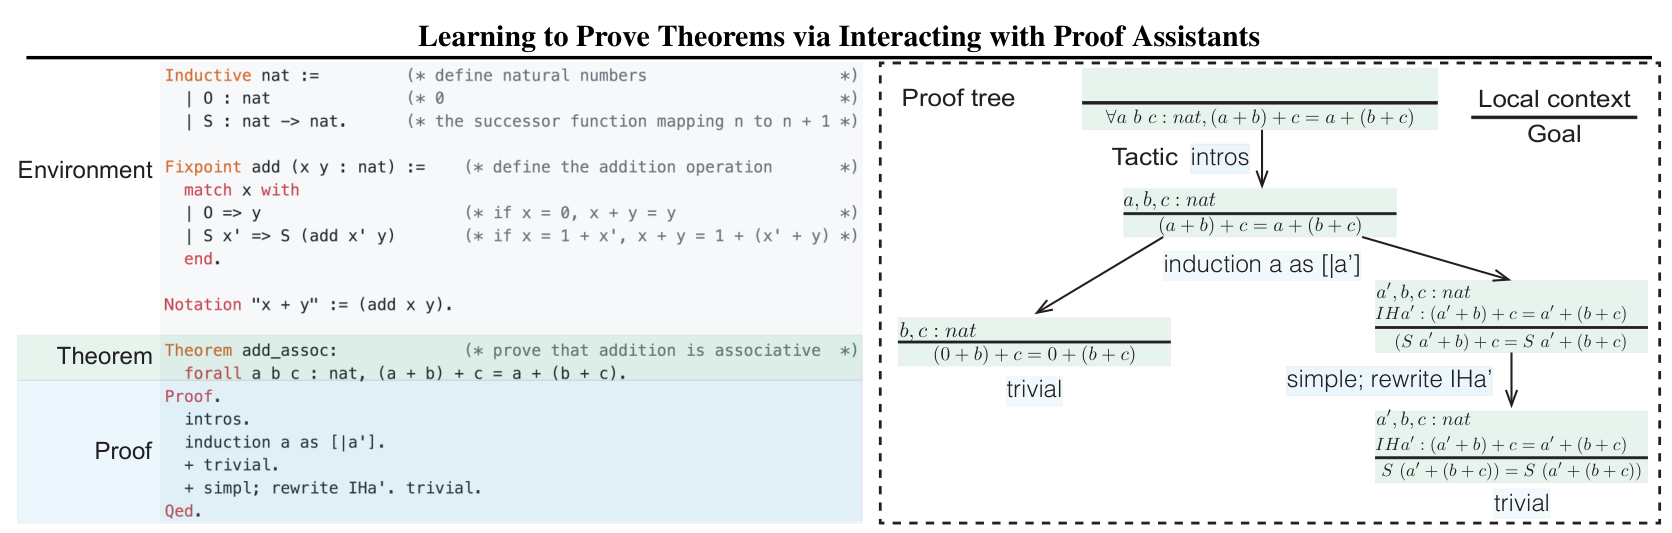
\includegraphics[width=1\textwidth]{images/proof_assistant_example.png}
    \caption{Automated Proof Assistant: example for induction "tactic" \cite{coqgym}}
    \label{fig:atp}
\end{figure}

\subsection{Automated Theorem Proving and Dataset}
\textbf{Automated Theorem Proving}: Automated Theorem Proving (ATP) refers to using a system or agent to automatically construct mathematical proofs for a given statement. Most of these systems have some representation of the environment (currently defined variables and types), available premises, and proof tactics (i.e. induction). The objective of an ATP agent is to select effective tactics in combination with premises and their arguments to decompose a goal into subgoals, recursively, until all subgoals under a target goal have been resolved. A goal is considered ``proved'' when all subgoals return empty lists of subgoals.

The fundamental difficulty is that the space of trees grows exponentially and the query time for applying a tactic is not insignificant, both of which easily lead to infeasible training times. Learning to effectively search over this domain is the objective of ATP agents. While the built-in ``auto'' mode in Coq can prove 2.9\% of theorems in the CoqGym (detailed below) benchmark, recent neural-augmented ATP systems have significantly outperformed this mode. Inspired by recent papers on neural-powered ATP systems, we hope to improve on some of these benchmarks with Graph Neural Networks (GNNs). We hope to construct improved graph embeddings for goals and premises using hierarchical GNNs with differential pooling. Given sufficient time, we also hope to replace LSTM and GRU attention modules with modern transformers.

\textbf{Dataset}: The dataset we would use is embedded in the environment
\texttt{CoqGym} and consists of 70,856 human-written proofs. For training
purposes, the authors also extracted approximately 160,000 one-step proofs,
110,000 two-step proofs, and 80,000 three-step proofs, and 61,000 four-step
proofs. The average number of steps per complete proof was 9.1.

\section{Graph ML techniques}
\subsection{Literature review}
\textbf{CoqGym} \cite{coqgym}: The model architecture for \texttt{CoqGym} can be separated into two parts: (a) Coq term (goals and premises) encoder, and (b) tactic decoder. A summary of the model is shown in Figure \ref{fig:coq_arch}.

The encoder embeds the current goal and any premises included in the local context or environment. The goal and premise statements are stored in graph structures known as abstract syntax trees (ASTs). These ASTs are then encoded into feature vectors using a \texttt{TreeLSTM} network \cite{TreeLSTM}. The feature vector output is created by concatenating the hidden state of the tree root with a 3-dim one-hot vector that indicates whether the term is a goal, environment premise or context premise.

The decoder predicts the "next best tactic" given the embeddings of our inputs: current goal, local context and environment. Under the hood, \texttt{CoqGym} implements a gated recurrent unit (GRU) with an attention module. Attention in this context helps the GRU attend more to the relevant assumptions (premises) from the context and environment lists since many will just be noise for any given goal. The GRU outputs a state vector $\vec{s}_t$ which is then passed through a softmax to produce a probability distribution over the set of potential tactics  $\vec{p}_t$ \footnote{$\vec{p}_t = \text{softmax} (W_R \cdot f(\vec{s}_t)$, where $f$ is a tanh (linear layer) and $W_R$ is the embedding matrix for production rules. }. The highest probability tactic is then applied to the current goal (sent to the prover along with context and environment) and we repeat the exercise for the returned subgoal(s). 

\begin{figure}[H]
    \centering
    % Kind of small for coq architecture, not sure if that matters much
    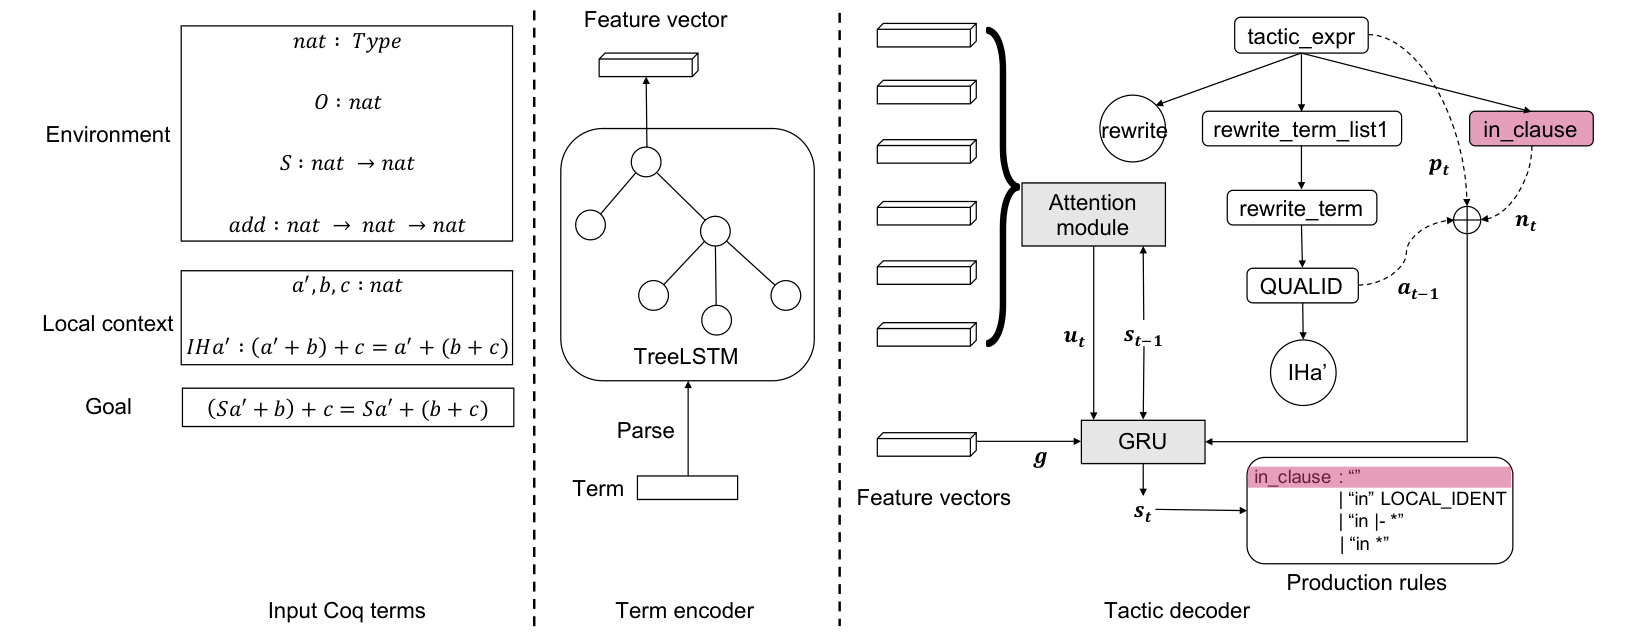
\includegraphics[width=1\textwidth]{images/coqgym.png}
    \caption{CoqGym model architecture \cite{coqgym}}
    \label{fig:coq_arch}
\end{figure}

\textbf{HOList} \cite{hol}: The \texttt{HOList} model can similarly be separated into two parts: (a) the goal and premise encoder, and (b) the tactic and premise chooser. A summary of this model is shown in Figure \ref{fig:hol_arch}.

The model architecture that Paliwal et al. proposed leverages the natural tree structure  of higher order logic (HOL) represented using S-expressions. They proposed multiple graph modifications to reduce the size of the graph (leaf sharing, sub-expression sharing, directed edges) to help reduce the size of the graphical representations. Using these graphs, they created two GNNs of the same structure with different weights to transform the goals and premises from trees to embeddings. Each GNN hop (with a $k$ hop hyperparameter) consisted of a MLP message passing layer, an average aggregation layer, and a $\texttt{SUM}(\texttt{self}, \texttt{MLP}\texttt{concat}(\texttt{AVG}, \texttt{self}))$ update function. Finally, the embeddings were calculated through a 1$\times$1 convolution with max pooling over the nodes of the tree.

The goal embeddings are then to classify a set of $k_1 = 5$ appropriate tactics, which is then used to rank the top $k_2 = 20$ valid premises to use as arguments for the tactics. These tactics are then sent into the proving assistant to retrieve the next set of goals and additional premises. 

\begin{figure}[H]
    \centering
    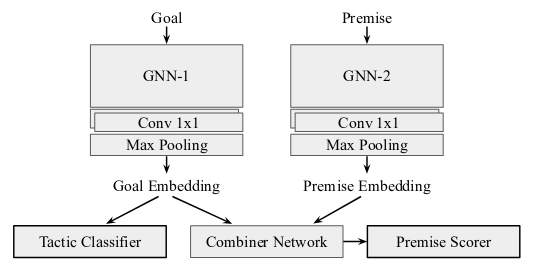
\includegraphics[width=0.7\textwidth]{images/HOL_model_architecture.png}
    \caption{HOL model architecture \cite{hol}}
    \label{fig:hol_arch}
\end{figure}

\subsection{Proposed method}
% Which graph ML model are you planning to use?
% Describe the model (try using figures and equations).
% Why is the model appropriate for the dataset you have chosen?
Our approach consists of translating proofs represented as \texttt{Coq} abstract syntax trees into PyGeometric graphs and using Graph Convolutional Networks (GCNs) to create embeddings for each proof tree. There will be a prediction head after the GCN to predict valid tactics, conditional on the input goal tree. Our supervised data will consist of human-proved Coq statements from CoqGym, and we will use cross-entropy loss to propagate errors back to the embeddings. Our design hopes to combine some of the stronger elements of both \cite{hol} and \cite{coqgym} to improve overall performance. In particular, our first objective is to replace the TreeLSTM in CoqGym with the GNN used by \cite{hol}. Unlike \cite{hol}, however, we will use the more expressive Coq AST as the input to our GNN encoder. We hope to further improve performance over \cite{hol} by using differential pooling \cite{hier} instead of convolution-max pooling. Lastly, given sufficient time, we would like to replace the GRU attention module in CoqGym with a transformer for improved attention over the goal and premise embeddings. We believe these architectural choices best exploit the structure of proof trees and the relationships between goals, premises, and tactics.

We will evaluate our model on the same benchmark as the CoqGym paper \cite{coqgym} using success rate or the number of successfully proved statements over the total number attempted.

\subsection{Risks \& open questions}
There are several risks we have tried to mitigate over the past week through literature review and tinkering in the \texttt{Coq} environment. In particular:
\begin{itemize}
    \item \textbf{Domain knowledge}: Not everyone in the group has a background
      in theoretical math or theorem proving. No one in the group has used Coq
      before.
      
    \item \textbf{Training time}: If we set the proof timeout at 20 seconds, it would take approximately 16 days to run over the entire dataset of 71,000 proofs. Accordingly, we will need to select a subset of proofs to iterate on before training the full model. It might also be possible to train our encoder (embeddings) independently of the decoder model.
    % However, we believe that we can train the graph neural network representations independently of the agent that interacts with the ATP, since these embeddings are based on graph structure.
\end{itemize}


\printbibliography

\end{document}


